%-----------------------------------------------------------
% These packages are essential to produce the poster
%-----------------------------------------------------------
\usepackage[scale=1.24]{beamerposter}
\usepackage{graphicx,amsfonts}
\usepackage{pdfpages}
\usepackage{subcaption}
\newcounter{figura}
\setcounter{figura}{1}

%-----------------------------------------------------------
% Custom commands that I use frequently
%-----------------------------------------------------------
\newcommand{\bb}[1]{\mathbb{#1}}
\newcommand{\cl}[1]{\mathcal{#1}}
\newcommand{\fA}{\mathfrak{A}}
\newcommand{\fB}{\mathfrak{B}}
\newcommand{\Tr}{{\rm Tr}}
\newtheorem{thm}{Theorem}
\newcommand{\captione}[2]{\begin{minipage}[l]{#1}\begin{center} \textit{Figure \thefigura.}\  #2\end{center}\end{minipage}\addtocounter{figura}{1}}
\newcommand{\spacer}{\begin{column}{\sepwid}\end{column}}
\newcommand{\toplogo}[2]{\newcommand{\posterlogo}{\includegraphics[width=#1]{mypics/#2}}}
\newcommand{\extrainfo}[1]{\newcommand{\inforight}{#1}}
\newcommand{\moreinfo}[1]{\newcommand{\inforightother}{#1}}
\newcommand{\conjetura}[2]{\\[-8mm]\begin{minipage}[l]{45cm}\emph{#1}\end{minipage}& \,\hspace{2cm} \emph{#2}\hspace{2cm}\,\\[-6mm]  \\ \hline}


%-------------------------------------------------------------------------------------------------------------------------------
% These commands will help me to build new blocks, do not modify!
%-------------------------------------------------------------------------------------------------------------------------------

\def\newblock#1#2#3{\expandafter\def\csname Block#1\endcsname{\begin{block}{#2}\rmfamily{#3}\end{block}}}
\def\newAlert#1#2#3{\expandafter\def\csname Alert#1\endcsname{\begin{alertblock}{#2}\rmfamily{#3}\end{alertblock}}}
\def\newSingle#1#2{\expandafter\def\csname Single#1\endcsname{\begin{column}{\onecolwid}#2\end{column}}}
\def\newMarried#1#2{\expandafter\def\csname Married#1\endcsname{\begin{column}{\twocolwid}#2\end{column}}}
\def\newTwin#1#2{\expandafter\def\csname Twin#1\endcsname{\begin{columns}[t,totalwidth=\twocolwid]#2\end{columns}}}





%-----------------------------------------------------------
% Define the column width and poster size
% To set effective sepwid, onecolwid and twocolwid values, first choose how many columns you want and how much separation you want between columns
% The separation I chose is 0.024 and I want 4 columns
% Then set onecolwid to be (1-(4+1)*0.024)/4 = 0.22
% Set twocolwid to be 2*onecolwid + sepwid = 0.464
%-----------------------------------------------------------

\newlength{\sepwid}
\newlength{\onecolwid}
\newlength{\twocolwid}
\setlength{\paperwidth}{48in}
\setlength{\paperheight}{36in}
\setlength{\sepwid}{0.024\paperwidth}
\setlength{\onecolwid}{0.22\paperwidth}
\setlength{\twocolwid}{0.464\paperwidth}
\setlength{\topmargin}{-0.5in}
\usetheme{confposter}

%-----------------------------------------------------------
% Define colours (see beamerthemeconfposter.sty to change these colour definitions)
%-----------------------------------------------------------

\setbeamercolor{block title}{fg=ngreen,bg=white}
\setbeamercolor{block body}{fg=black,bg=white}
\setbeamercolor{block alerted title}{fg=white,bg=dblue!70}
\setbeamercolor{block alerted body}{fg=black,bg=dblue!10}






%-----------------------------------------------------------------------------------------------------------------------------------------
%                               START TYPING YOUR BLOCKS !!
%-----------------------------------------------------------------------------------------------------------------------------------------
%%%%%%%%%%%%%%%%%%%%%%%%%%%%%%%%%%%%%%%%%%%%%  IMPORTANT %%%%%%%%%%%%%%%%%%%%%%%%%%%%%%%%%%%%%%%%%%%%%%%%%%%%%%%%%%%%%%%%%%%%%%%%%%%%%%%%%
%%%%%%%%%%%%%%%%%%%%%%%%%%%%%%%%%%%%%%%%%%%%%  IMPORTANT %%%%%%%%%%%%%%%%%%%%%%%%%%%%%%%%%%%%%%%%%%%%%%%%%%%%%%%%%%%%%%%%%%%%%%%%%%%%%%%%%
%%%   NO EMPTY ROWS. This example shows what you are NOT to do:
%%%  \newAlert{Main}{Main First Example}{
%%%             This is the main topic, blah blah blah
%%%
%%%             and then blah blah blah
%%%             }
%%%%%%%%%%%%%%%%%%%%%%%%%%%%%%%%%%%%%%%%%%%%%%%%%%%%%%%%%%%%%%%%%%%%%%%%%%%%%%%%%%%%%%%%%%%%%%%%%%%%%%%%%%%%%%%%%%%%%%%%%%%%%%%%%%%%%%%%%%
















%%%%%%%%%%%%%%%%%%%%%%%%%%%%%%%%%%%%%%%%%%%%%%%%%%%%%%%%%%%%%%%%%%%%%%%%%%%%%%%%%%%%%%%%%%%%%%%%%%%%%%%%%%%%%%%%%%%%%%%%%%%%%%%%%%%%%%%%%%%
%%%%%%%%%%%%%%%%%%%%%%%%%%%%%%%%%%%%%%%%%%%%%%%%%%%%%%%%%%%%%%%%%%%%%%%%%%%%%%%%%%%%%%%%%%%%%%%%%%%%%%%%%%%%%%%%%%%%%%%%%%%%%%%%%%%%%%%%%%%
%%%%%%%%%%%%%%%%%%%%%%%%%%%%%%%%%%%%%%%%%%%%             REGULAR    BLOCKS  START          %%%%%%%%%%%%%%%%%%%%%%%%%%%%%%%%%%%%%%%%%%%%%%%%
%%%%%%%%%%%%%%%%%%%%%%%%%%%%%%%%%%%%%%%%%%%%%%%%%%%%%%%%%%%%%%%%%%%%%%%%%%%%%%%%%%%%%%%%%%%%%%%%%%%%%%%%%%%%%%%%%%%%%%%%%%%%%%%%%%%%%%%%%%%
%%%%%%%%%%%%%%%%%%%%%%%%%%%%%%%%%%%%%%%%%%%%%%%%%%%%%%%%%%%%%%%%%%%%%%%%%%%%%%%%%%%%%%%%%%%%%%%%%%%%%%%%%%%%%%%%%%%%%%%%%%%%%%%%%%%%%%%%%%%




%%%%%%%%%%%%%%%%%%%%%%%%%%%%%%%%%%%%%%%%%%%%%%%%%%%%%%%%%%%%%%%%%%%%%%%%%%%%%%%%%%%%%%%%%%%%%%%%%%%%%%%%%%%%%%%%%%%%%%%%%%%%%%%%%%%%%%%%%%%
\newblock{Introduction}{Introduction}{
        The purpose of our research is to study distributed search-and-evacuation algorithms.
        These algorithms involve mobile agents (or robots) searching in geometric domains, such as a closed disk or a convex polygon.
        By working together and communicating with one another, the mobile agents search for an exit hidden on the perimeter.
        The goal of our research is to create and study exit strategies that terminate as quickly as possible.
        }
%%%%%%%%%%%%%%%%%%%%%%%%%%%%%%%%%%%%%%%%%%%%%%%%%%%%%%%%%%%%%%%%%%%%%%%%%%%%%%%%%%%%%%%%%%%%%%%%%%%%%%%%%%%%%%%%%%%%%%%%%%%%%%%%%%%%%%%%%%%








%%%%%%%%%%%%%%%%%%%%%%%%%%%%%%%%%%%%%%%%%%%%%%%%%%%%%%%%%%%%%%%%%%%%%%%%%%%%%%%%%%%%%%%%%%%%%%%%%%%%%%%%%%%%%%%%%%%%%%%%%%%%%%%%%%%%%%%%%%%
\newblock{Definitions}{Definitions}{
         \begin{description}[font=$\bullet$~\normalfont\textbf{}]
             \item[$\bullet$ An Exit] is a point unknown to the agents, that is located on the perimeter of a disk.
             \item[$\bullet$ Priority Agents] P1 and P2.
             \item[$\bullet$ A Helper] H, is an agent that simply assists the priority agents in finding the exit.
             \item[$\bullet$ Algorithm Termination] occurs if either P1 or P2 reaches the exit.
         \end{description}
         }
%%%%%%%%%%%%%%%%%%%%%%%%%%%%%%%%%%%%%%%%%%%%%%%%%%%%%%%%%%%%%%%%%%%%%%%%%%%%%%%%%%%%%%%%%%%%%%%%%%%%%%%%%%%%%%%%%%%%%%%%%%%%%%%%%%%%%%%%%%%








%%%%%%%%%%%%%%%%%%%%%%%%%%%%%%%%%%%%%%%%%%%%%%%%%%%%%%%%%%%%%%%%%%%%%%%%%%%%%%%%%%%%%%%%%%%%%%%%%%%%%%%%%%%%%%%%%%%%%%%%%%%%%%%%%%%%%%%%%%%
\newblock{Description}{Algorithm Description}{
         %In our algorithm, we use two \textbf{priority} agents and one \textbf{helper} agent.
         %The termination condition in our algorithm is reached when either one of the two priority agents reaches the exit.
         % INCLUDE A FRAME OF REFERENCE. 0 DEGREES IS AT 3:00. %
         %We send one priority and one helper to some angle $\alpha$ on the perimeter of the shape, in the third quadrant.
         %The priority agent travels counter-clockwise, and the helper travels clockwise.
         %The other priority agent travels to 0 radians and travels counter-clockwise.
         % INCLUDE A FRAME OF REFERENCE. 0 DEGREES IS AT 3:00. %
         \begin{description}[font=$\bullet$~\normalfont\textbf{}]
             \item[$\bullet$] The priority agents are \textbf{P1 and P2}. The helper agent is \textbf{H}.
             \item[$\bullet$] \textbf{P2} along with \textbf{H} go at angle $\alpha$ in the third quadrant to the perimeter. \textbf{H} travels clockwise, and \textbf{P2} travels counterclockwise.
             \item[$\bullet$] \textbf{P1} travels at angle 0 to the perimeter, and travels counterclockwise.
             \item[$\bullet$] The algorithm is required to ensure that between the agents,
             every part of the perimeter will potentially get searched before the exit is found.
         \end{description}
         }

 \newblock{DescriptionDos}{Algorithm Steps}{
          \captionsetup[figure]{labelformat=empty}
          \begin{figure}
              \centering
              %\begin{subfigure}
              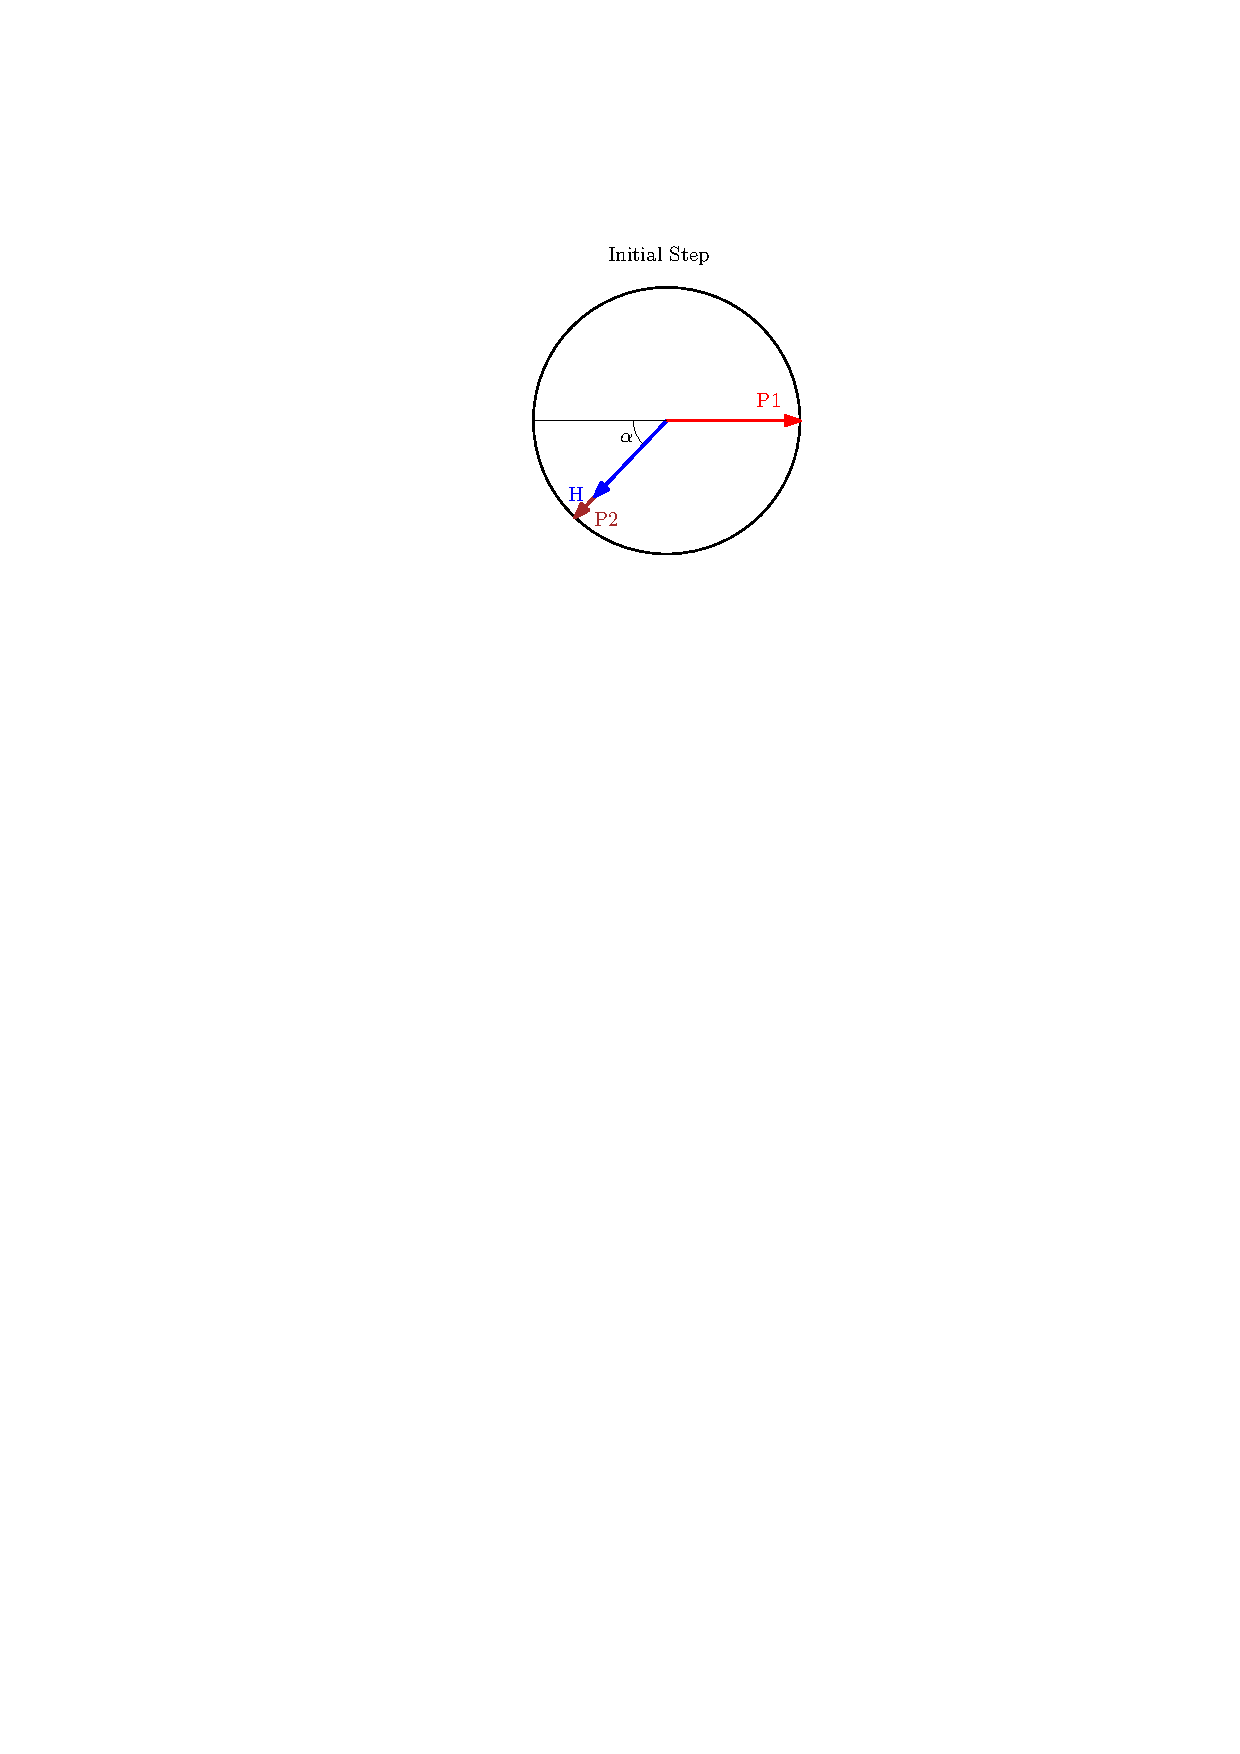
\includegraphics[width=0.53\textwidth]{mypics/2Q1S_Initial.pdf}
              %\caption{Figure 1}
              %\end{subfigure}
              %\begin{subfigure}
              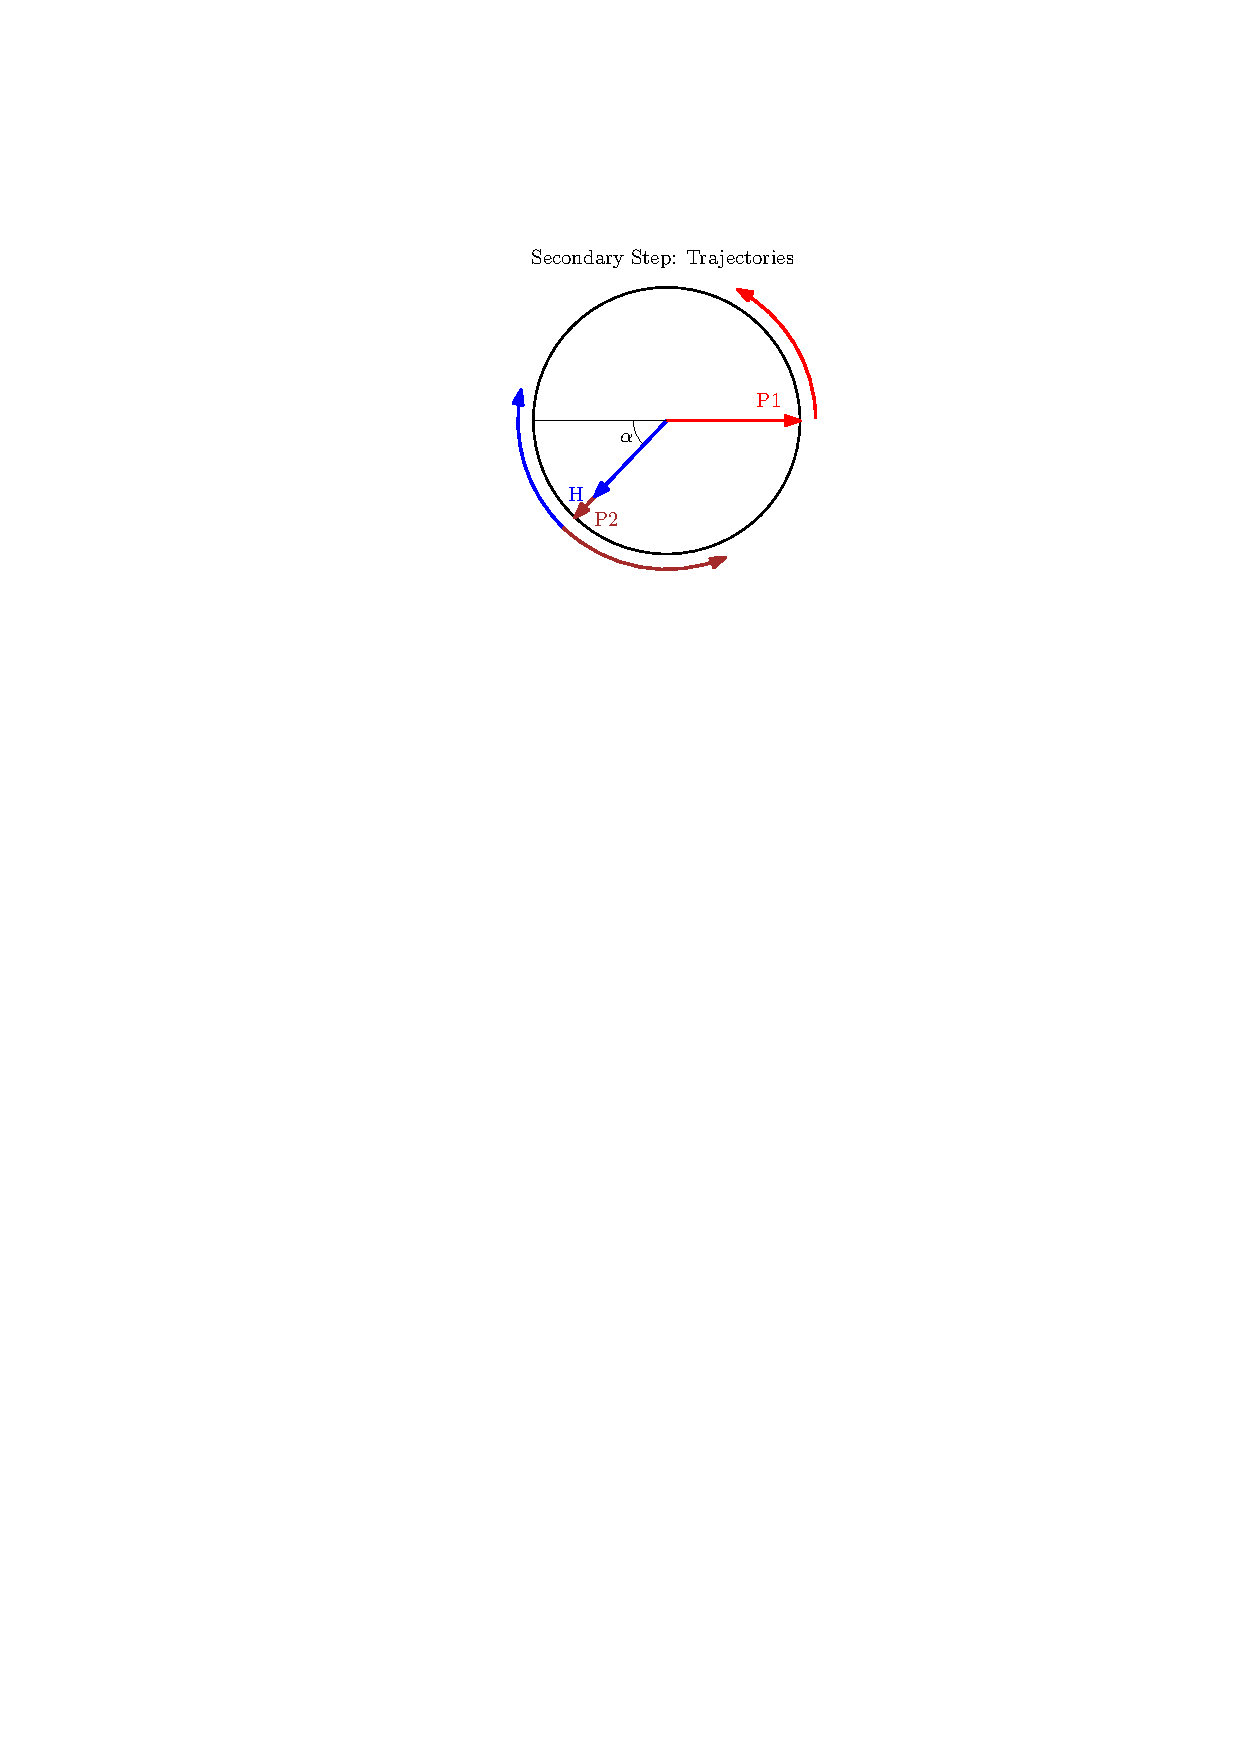
\includegraphics[width=0.45\textwidth]{mypics/2Q1S_Second_Step.pdf}
              %\caption{Figure 2}
              %\end{subfigure}
          \end{figure}
          }
%%%%%%%%%%%%%%%%%%%%%%%%%%%%%%%%%%%%%%%%%%%%%%%%%%%%%%%%%%%%%%%%%%%%%%%%%%%%%%%%%%%%%%%%%%%%%%%%%%%%%%%%%%%%%%%%%%%%%%%%%%%%%%%%%%%%%%%%%%%

%	the exit is unknown, and that this is an animation of a distributed algorithm,
%	and in the is distibuted algoirithm, we have a multiple bots trying to find an  exit,
%	where two are distinguished and one is a helper, where only one distinguish must reach.
%	crab.rutgers.edu/~shende/ rutgers library system first and search for them, or look through articles, by a link that says do you want an onlune version, which will give access to al l the source, as in the pdf, but not directly.
%	2018 God save the queen
%	fun with algorithms - god saves the queen
%




%%%%%%%%%%%%%%%%%%%%%%%%%%%%%%%%%%%%%%%%%%%%%%%%%%%%%%%%%%%%%%%%%%%%%%%%%%%%%%%%%%%%%%%%%%%%%%%%%%%%%%%%%%%%%%%%%%%%%%%%%%%%%%%%%%%%%%%%%%%
\newblock{Work}{Future Work}{
        This is an example of an algorithm that abstracts real world problems,
        where a specified subset of agents has to evacuate.
	    In the future we will study further distributed algorithms of search and evacuate on lines and polygons,
        or even topologies such as arbitrary finite graphs. To analyze these, we have created a web app that
        shows visualizations and helpful data of all of the algorithms that we have studied. Link to website: \textbf{https://bit.ly/2Vv85OJ}
        }
%%%%%%%%%%%%%%%%%%%%%%%%%%%%%%%%%%%%%%%%%%%%%%%%%%%%%%%%%%%%%%%%%%%%%%%%%%%%%%%%%%%%%%%%%%%%%%%%%%%%%%%%%%%%%%%%%%%%%%%%%%%%%%%%%%%%%%%%%%%










%%%%%%%%%%%%%%%%%%%%%%%%%%%%%%%%%%%%%%%%%%%%%%%%%%%%%%%%%%%%%%%%%%%%%%%%%%%%%%%%%%%%%%%%%%%%%%%%%%%%%%%%%%%%%%%%%%%%%%%%%%%%%%%%%%%%%%%%%%%
\newblock{Conclusions}{Conclusions}{
	This algorithm has an upper bound of 3.55 time units in the worst case. We can achieve this time by sending \textbf{H}
    and \textbf{P2} out at an angle of $\alpha = 5 \pi / 9 - 2\sqrt3 /3$, and $\beta = ( \pi / 3 - \alpha) / 2$,
    so that both of the worst case time predictions are equal.
       }
%%%%%%%%%%%%%%%%%%%%%%%%%%%%%%%%%%%%%%%%%%%%%%%%%%%%%%%%%%%%%%%%%%%%%%%%%%%%%%%%%%%%%%%%%%%%%%%%%%%%%%%%%%%%%%%%%%%%%%%%%%%%%%%%%%%%%%%%%%%

















%%%%%%%%%%%%%%%%%%%%%%%%%%%%%%%%%%%%%%%%%%%%%%%%%%%%%%%%%%%%%%%%%%%%%%%%%%%%%%%%%%%%%%%%%%%%%%%%%%%%%%%%%%%%%%%%%%%%%%%%%%%%%%%%%%%%%%%%%%%
\newblock{Bibliography}{References}{\small
      \begin{thebibliography}{99}
         \bibitem{} Jurek Czyzowicz, et. al., (2014). Evacuating Robots via Unknown Exit in a Disk. Proceedings of DISC 2014, LNCS 8784, pp. 122-136, 2014.
         \bibitem{} Jurek Czyzowicz, et. al., (2015). Evacuating Robots From a Disk Using Face-To-Face Communication. Proceedings of CIAC, 2015 p. 140-152, 2015.
         \bibitem{} Jurek Czyzowicz, et. al., Priority Evacuation from a Disk Using Mobile Robots, Proceedings of SIROCCO, pages 392-407, 2018.
         \bibitem{} Jurek Czyzowicz, et. al., God Save the Queen. Fun with Algorithms, arXiv:1804.06011v1 [cs.MA] 17 Apr 2018.
      \end{thebibliography}
      }
%%%%%%%%%%%%%%%%%%%%%%%%%%%%%%%%%%%%%%%%%%%%%%%%%%%%%%%%%%%%%%%%%%%%%%%%%%%%%%%%%%%%%%%%%%%%%%%%%%%%%%%%%%%%%%%%%%%%%%%%%%%%%%%%%%%%%%%%%%%













%%%%%%%%%%%%%%%%%%%%%%%%%%%%%%%%%%%%%%%%%%%%%%%%%%%%%%%%%%%%%%%%%%%%%%%%%%%%%%%%%%%%%%%%%%%%%%%%%%%%%%%%%%%%%%%%%%%%%%%%%%%%%%%%%%%%%%%%%%%
\newblock{Acknowledgements}{Acknowledgements}{\small
      This research is supported by the National Science Foundation under grant \# CCf-AF 1813940 (RUI: Search, Evacuation and Reconfiguration with Coordinated Mobile Agents).\vspace{0.2in}\hfill\break
      Our faculty advisor is Dr. Sunil Shende.
      }
%%%%%%%%%%%%%%%%%%%%%%%%%%%%%%%%%%%%%%%%%%%%%%%%%%%%%%%%%%%%%%%%%%%%%%%%%%%%%%%%%%%%%%%%%%%%%%%%%%%%%%%%%%%%%%%%%%%%%%%%%%%%%%%%%%%%%%%%%%%










%%%%%%%%%%%%%%%%%%%%%%%%%%%%%%%%%%%%%%%%%%%%%%%%%%%%%%%%%%%%%%%%%%%%%%%%%%%%%%%%%%%%%%%%%%%%%%%%%%%%%%%%%%%%%%%%%%%%%%%%%%%%%%%%%%%%%%%%%%%
\newblock{Logo}{}{\vspace{-4cm}
      \begin{center}
          
\includegraphics[width=1.5in]{mypics/temp.jpg}
      \end{center}
      }
%%%%%%%%%%%%%%%%%%%%%%%%%%%%%%%%%%%%%%%%%%%%%%%%%%%%%%%%%%%%%%%%%%%%%%%%%%%%%%%%%%%%%%%%%%%%%%%%%%%%%%%%%%%%%%%%%%%%%%%%%%%%%%%%%%%%%%%%%%%










%%%%%%%%%%%%%%%%%%%%%%%%%%%%%%%%%%%%%%%%%%%%%%%%%%%%%%%%%%%%%%%%%%%%%%%%%%%%%%%%%%%%%%%%%%%%%%%%%%%%%%%%%%%%%%%%%%%%%%%%%%%%%%%%%%%%%%%%%%%
%%%%%%%%%%%%%%%%%%%%%%%%%%%%%%%%%%%          REGULAR   BLOCKS     FINISH                   %%%%%%%%%%%%%%%%%%%%%%%%%%%%%%%%%%%%%%%%%%%%%%%%
%%%%%%%%%%%%%%%%%%%%%%%%%%%%%%%%%%%%%%%%%%%%%%%%%%%%%%%%%%%%%%%%%%%%%%%%%%%%%%%%%%%%%%%%%%%%%%%%%%%%%%%%%%%%%%%%%%%%%%%%%%%%%%%%%%%%%%%%%%%
















%%%%%%%%%%%%%%%%%%%%%%%%%%%%%%%%%%%%%%%%%%%%%%%%%%%%%%%%%%%%%%%%%%%%%%%%%%%%%%%%%%%%%%%%%%%%%%%%%%%%%%%%%%%%%%%%%%%%%%%%%%%%%%%%%%%%%%%%%%%
%%%%%%%%%%%%%%%%%%%%%%%%%%%%%%%%%%%%%%%%%%%%%%%%%%%%%%%%%%%%%%%%%%%%%%%%%%%%%%%%%%%%%%%%%%%%%%%%%%%%%%%%%%%%%%%%%%%%%%%%%%%%%%%%%%%%%%%%%%%
%%%%%%%%%%%%%%%%%%%%%%%%%%%%%%                  ALERT BLOCKS START                         %%%%%%%%%%%%%%%%%%%%%%%%%%%%%%%%%%%%%%%%%%%%%%%%
%%%%%%%%%%%%%%%%%%%%%%%%%%%%%%%%%%%%%%%%%%%%%%%%%%%%%%%%%%%%%%%%%%%%%%%%%%%%%%%%%%%%%%%%%%%%%%%%%%%%%%%%%%%%%%%%%%%%%%%%%%%%%%%%%%%%%%%%%%%
%%%%%%%%%%%%%%%%%%%%%%%%%%%%%%%%%%%%%%%%%%%%%%%%%%%%%%%%%%%%%%%%%%%%%%%%%%%%%%%%%%%%%%%%%%%%%%%%%%%%%%%%%%%%%%%%%%%%%%%%%%%%%%%%%%%%%%%%%%%


\newAlert{MainTopic}{Figures}{
                     \begin{center}
                         \begin{subfigure}
                             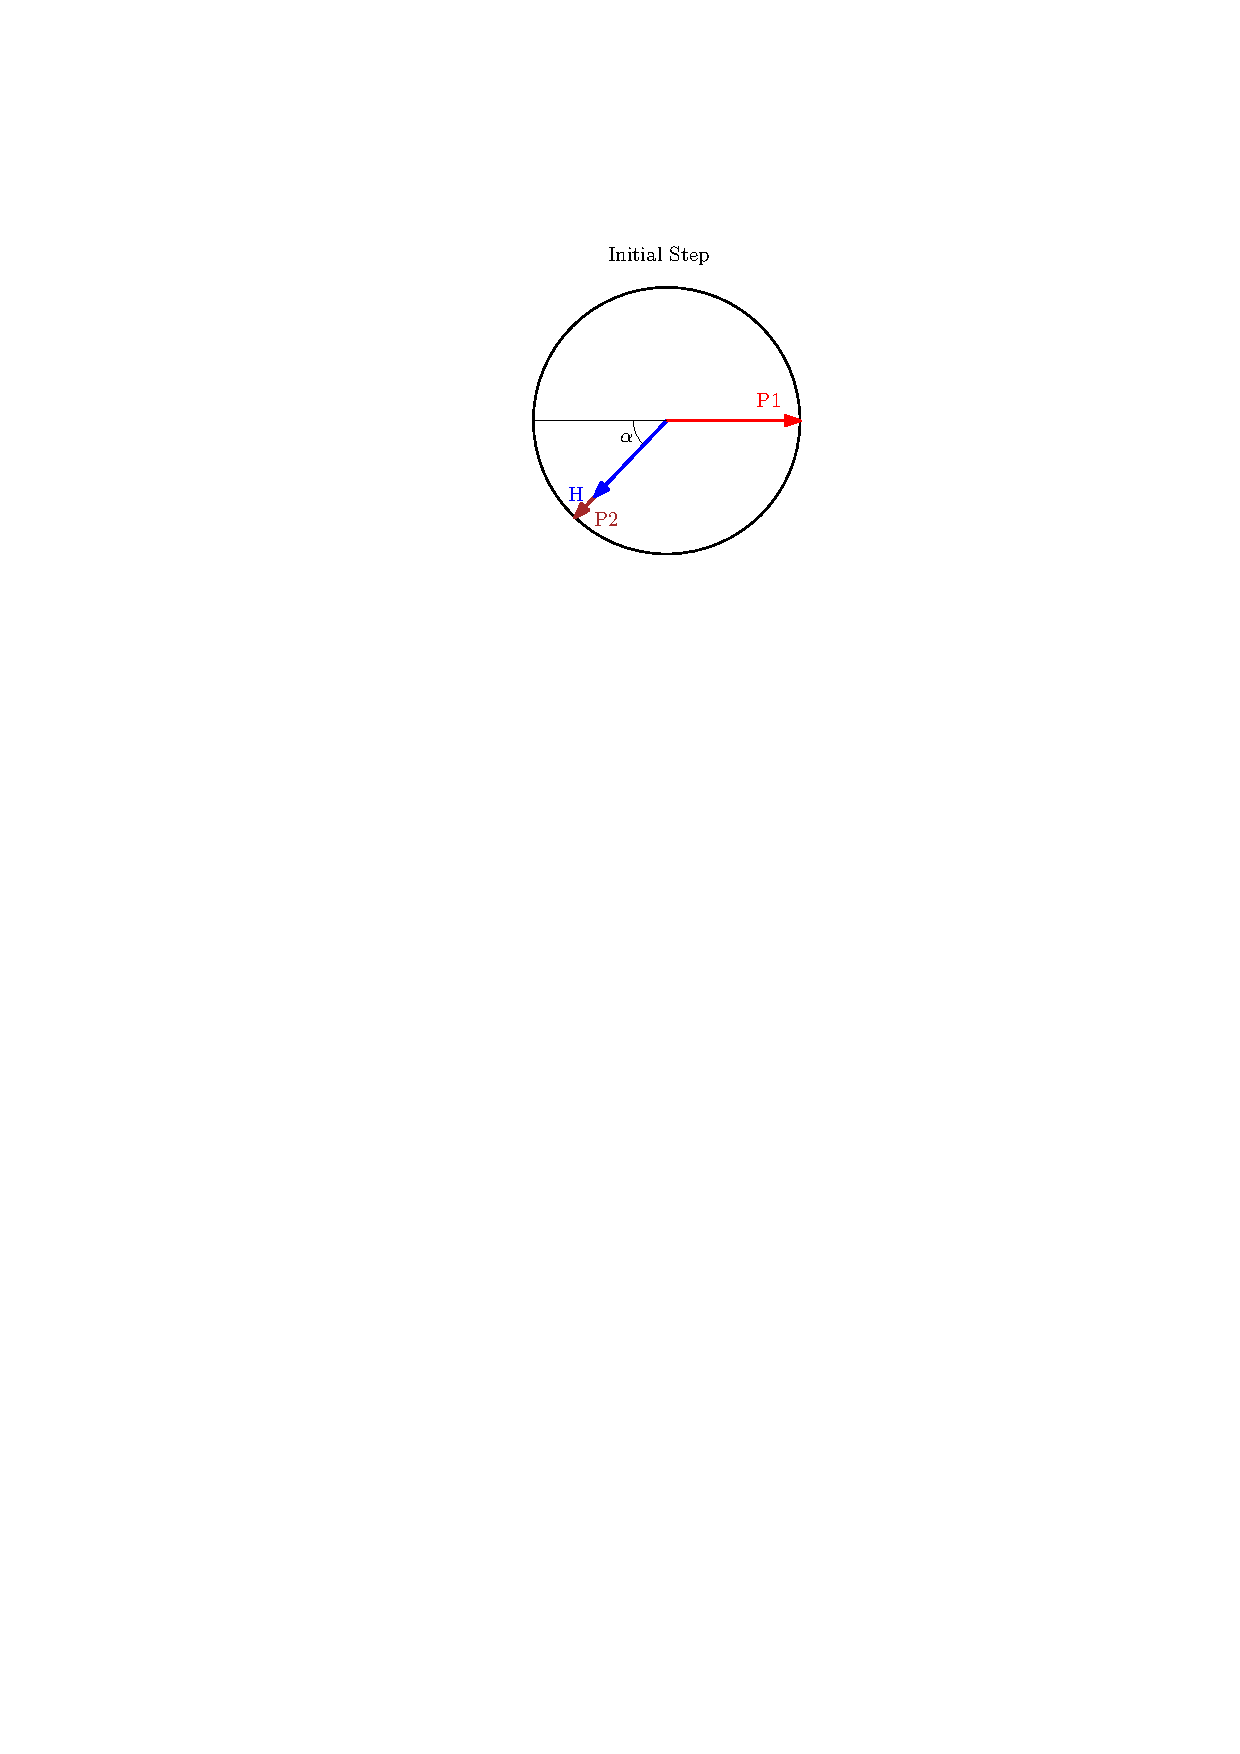
\includegraphics[width=0.23\textwidth]{mypics/2Q1S_Initial.pdf}
                         \end{subfigure}
                         \begin{subfigure}
                             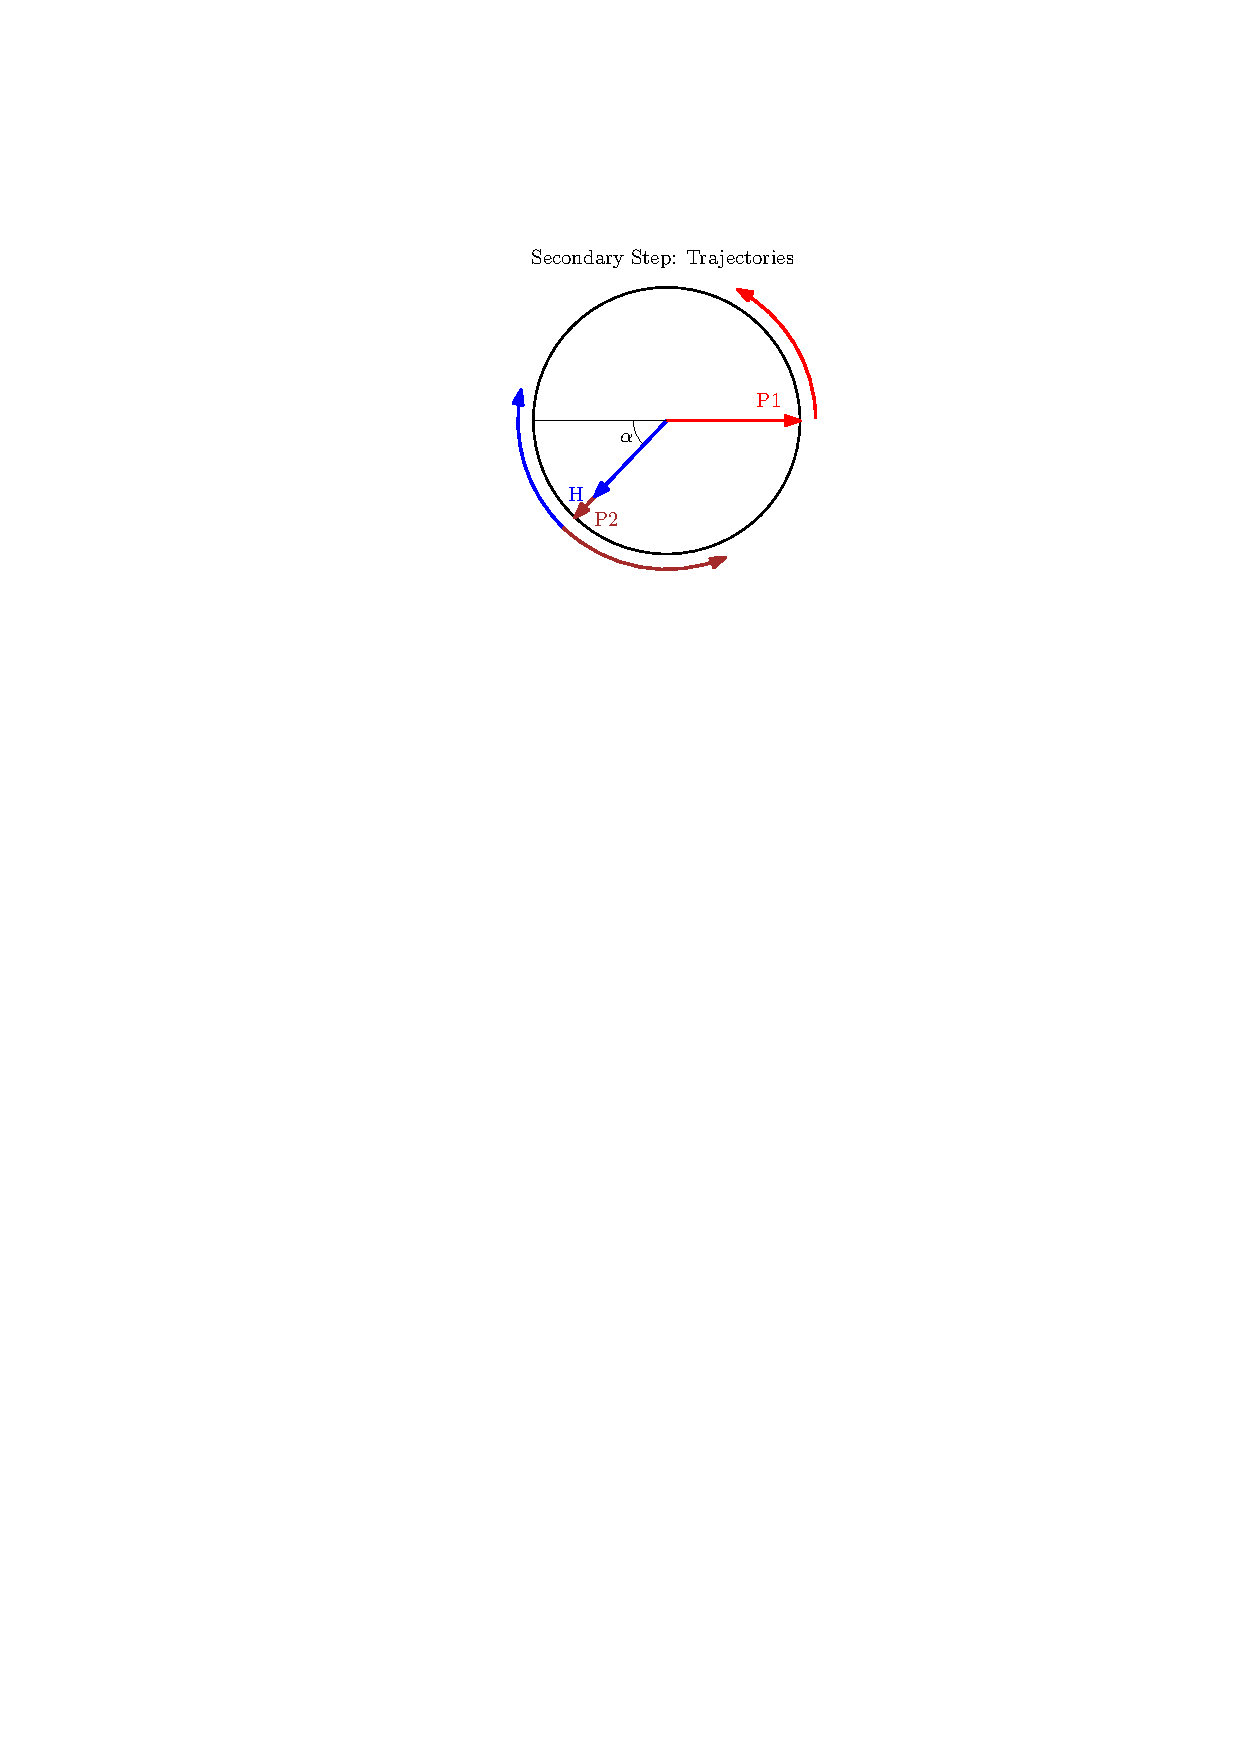
\includegraphics[width=0.2\textwidth]{mypics/2Q1S_Second_Step.pdf}
                         \end{subfigure}
                         \begin{subfigure}
                             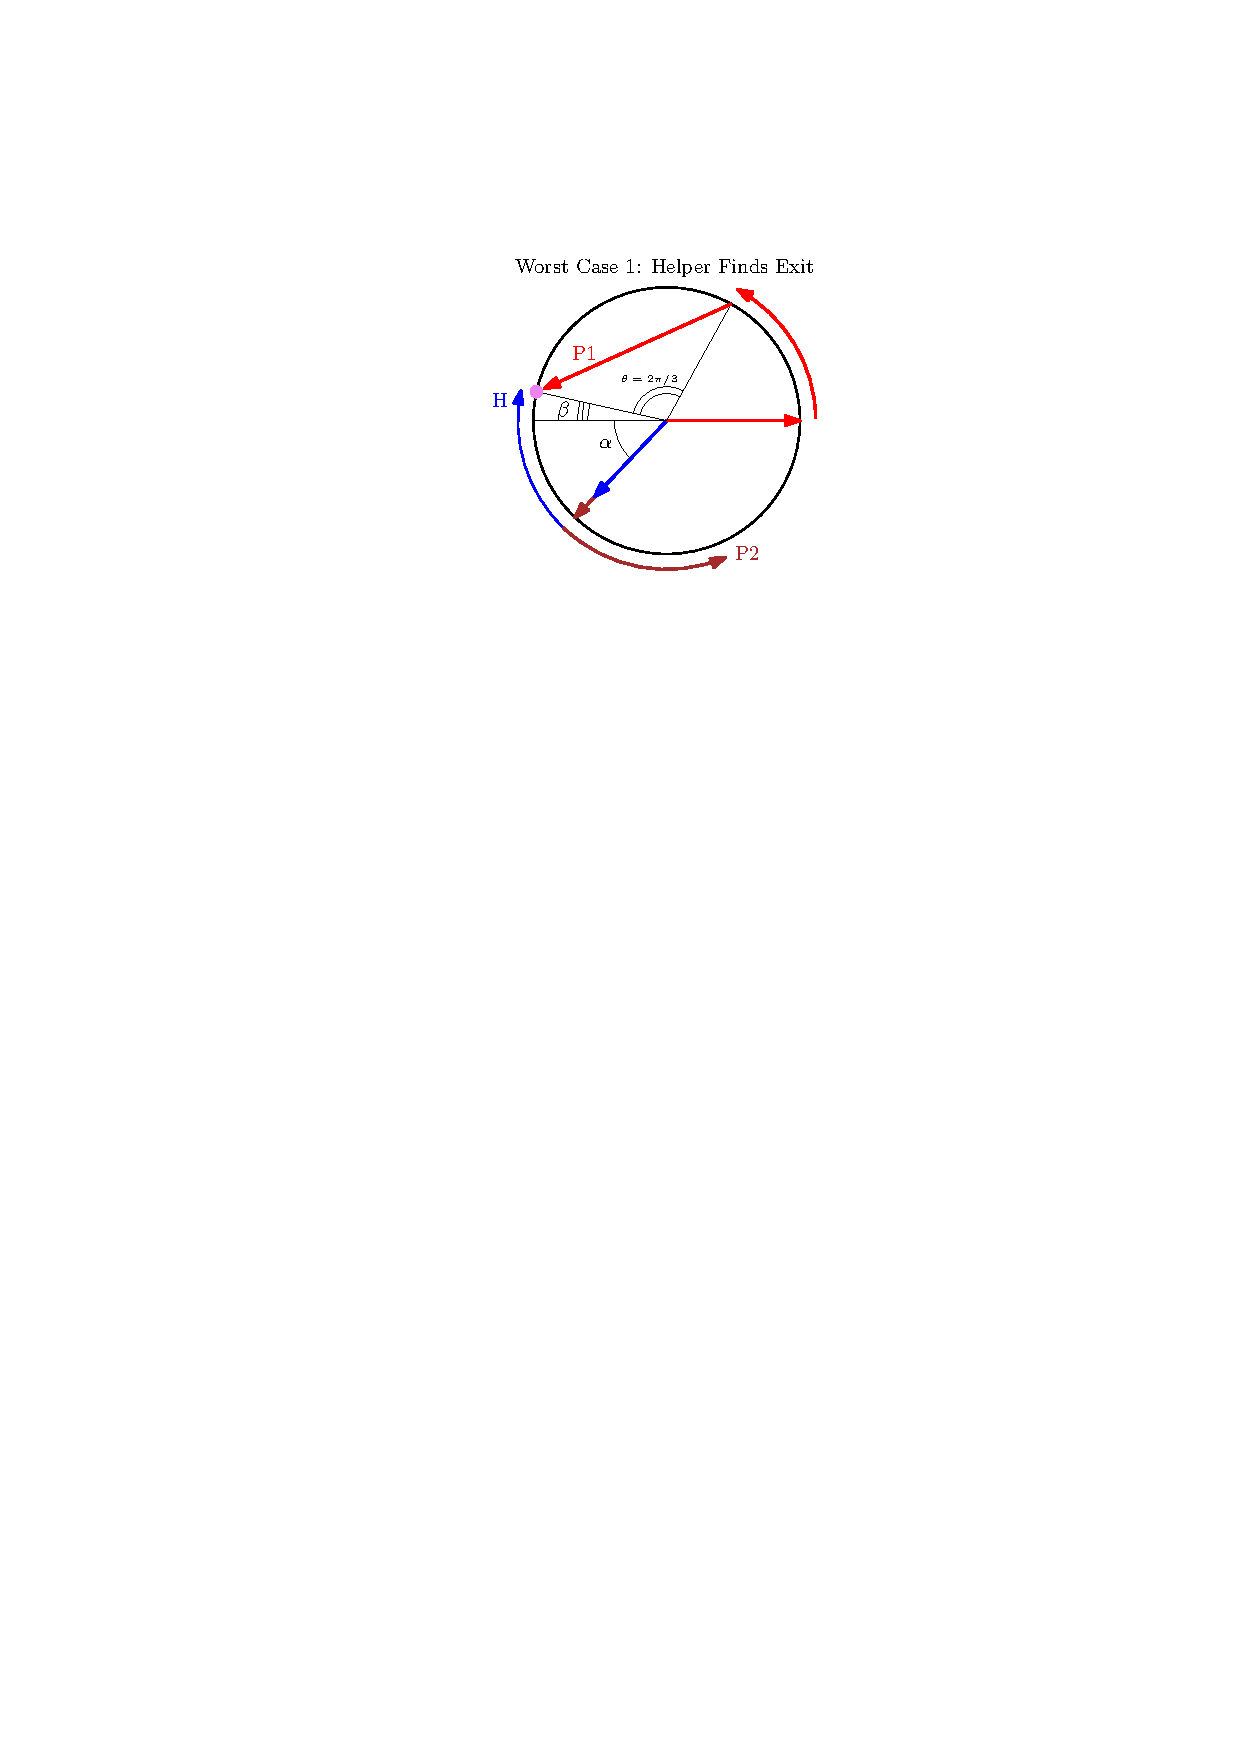
\includegraphics[width=0.22\textwidth]{mypics/2Q1S_WorstCase_Servant.pdf}
                         \end{subfigure}
                         \begin{subfigure}
                             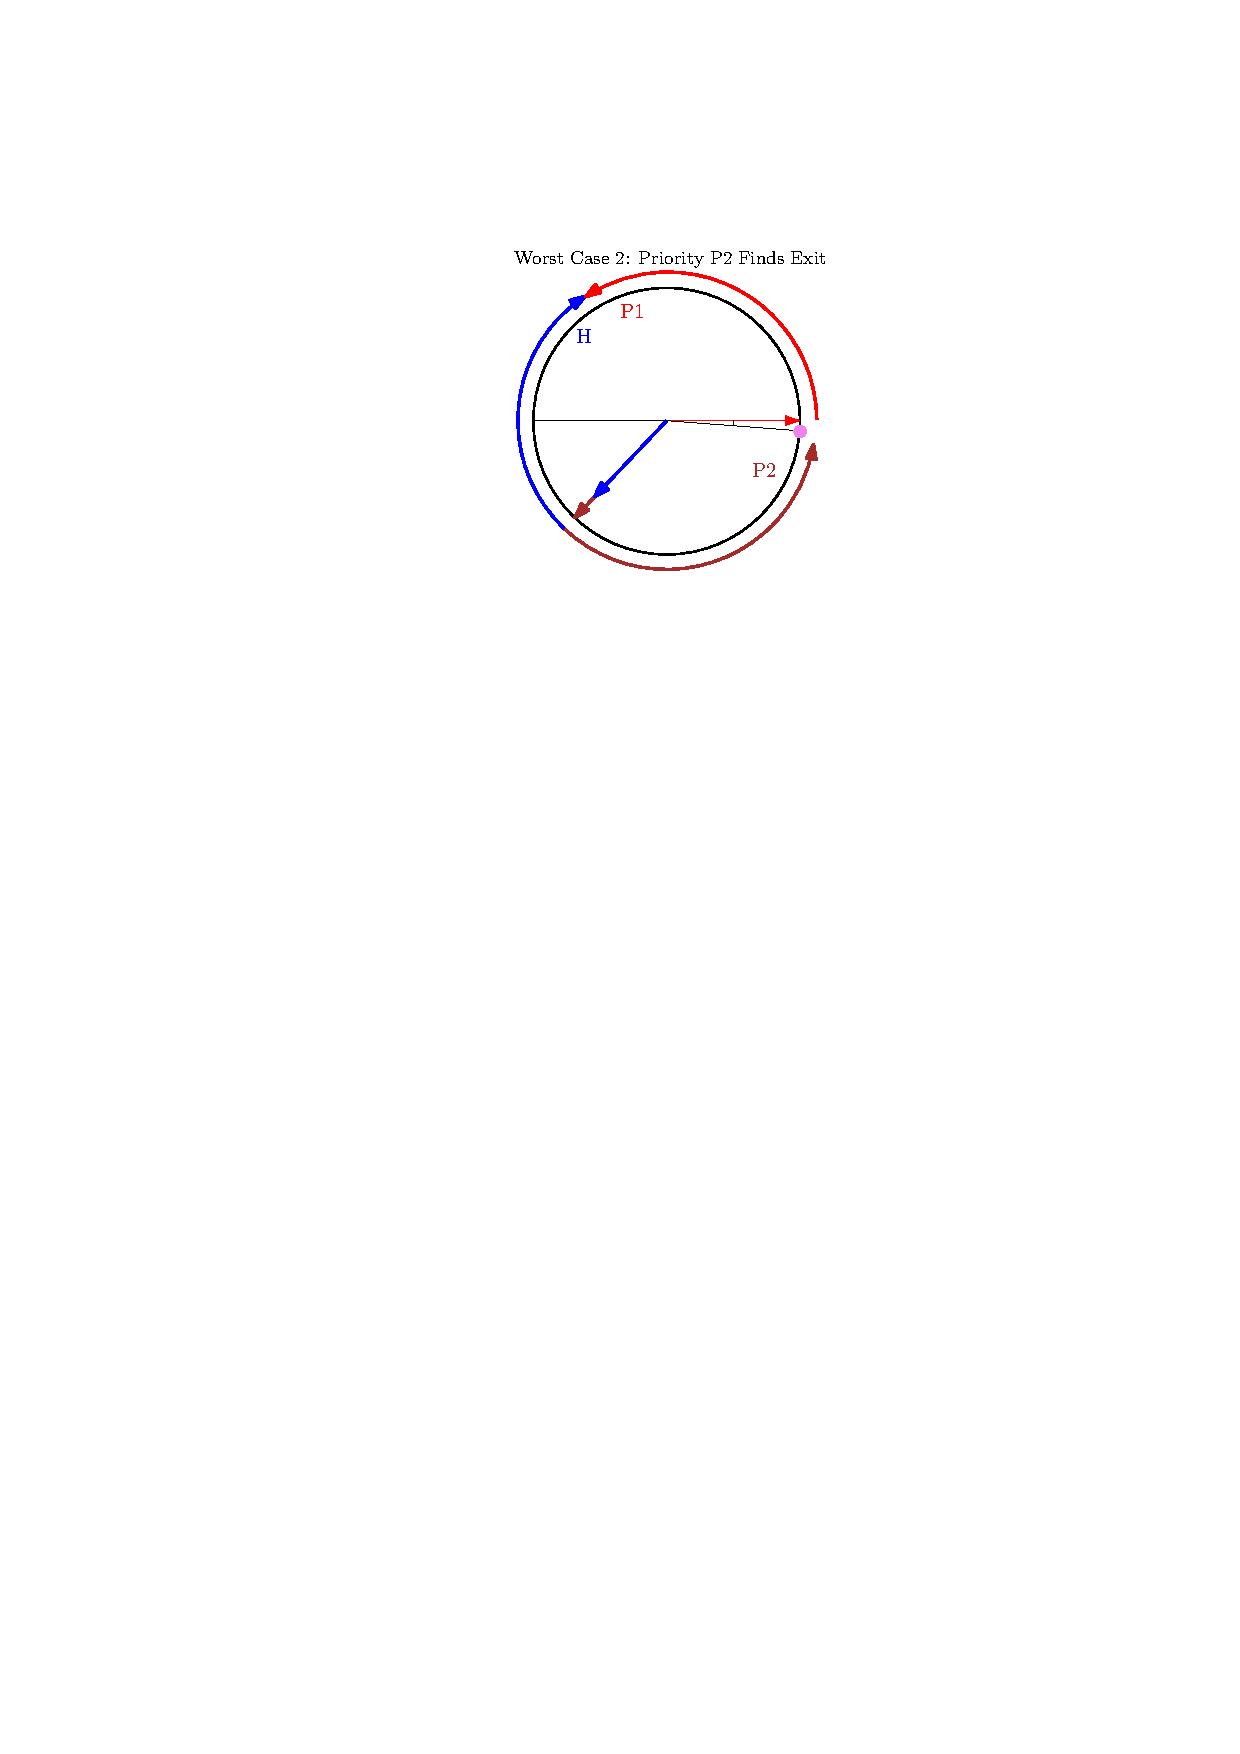
\includegraphics[width=0.2\textwidth]{mypics/2Q1S_WorstCase_Priority.pdf}
                         \end{subfigure}
                    \end{center}
            }

\newAlert{MainProblem}{Main Result}{
            The purpose of our research is to propose an algorithm for two
            priority agents and a helper agent to find an unknown
            exit on a disk. We show that this can be achieved in no more than
            3.55 time units in the worst case.
            \vspace{0.5in}
            \captionsetup[figure]{labelformat=empty}
            \begin{figure}
                \centering
                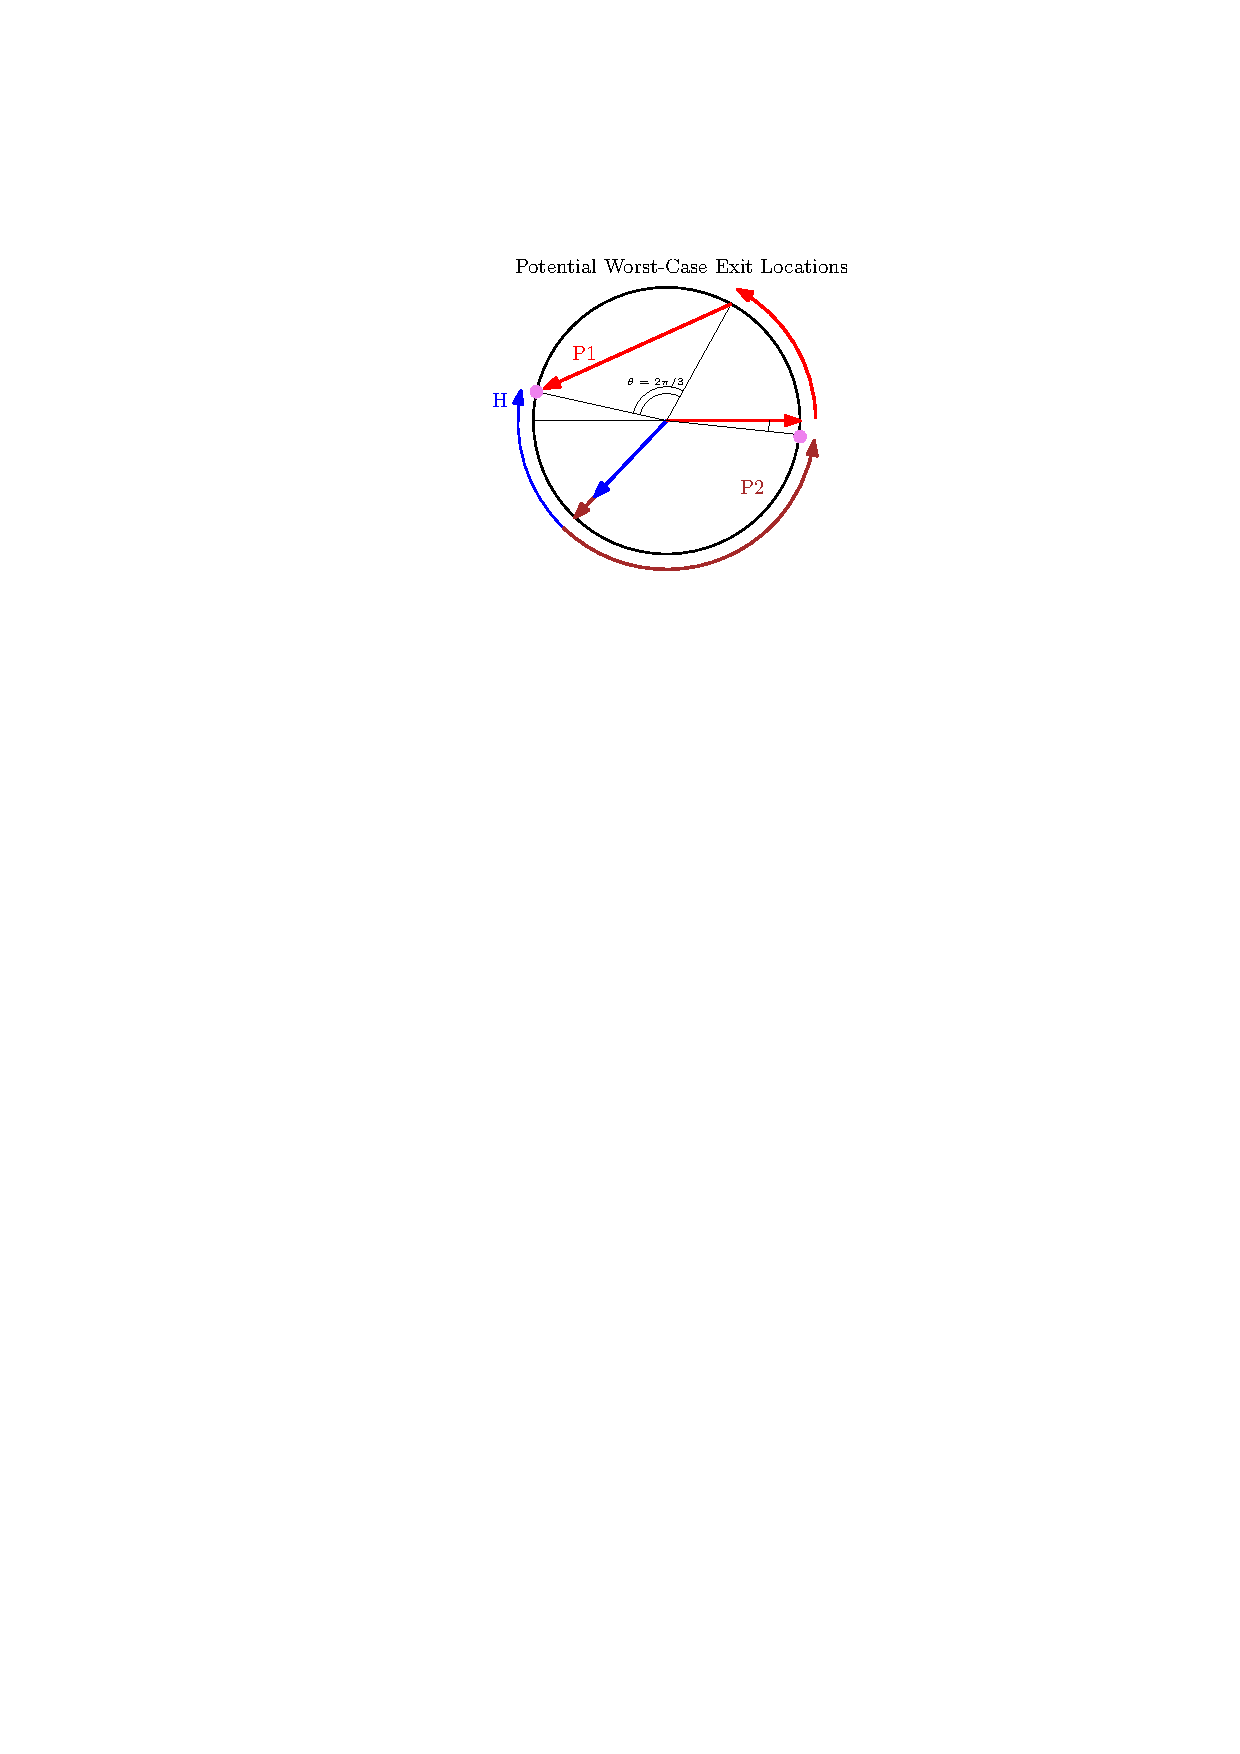
\includegraphics[width=0.6\textwidth]{mypics/2Q1S_WorstCase_Both.pdf}
                %\caption{Figure 3}
            \end{figure}
            }

\newAlert{Conjectures}{Our Analysis}{
            In this algorithm, we observe two worst case situations. In one, \textbf{P2} travels the entire distance
            of its arc, until it reaches the exit a small distance before 0 radians.
            In the other, \textbf{H} finds the exit at a point such that the closest priority
            agent (\textbf{P1}) would have to travel along a chord to reach it.\vspace{0.5in}\hfill\break % MAKE A NEW LINE WITH A SPACE
            We analyze the case in which \textbf{H} finds the exit in the second quadrant, at angle $\pi - \beta$.
            Say that there is an angle of $\theta$ between \textbf{P1} and \textbf{H}, such that
            the shortest distance between the two agents is $\[ 2 \sin (\theta / 2)$. The angle $\theta$ that
            would produce the longest distance between \textbf{P1} and \textbf{H}, is $\theta = 2 \pi / 3$.
            Therefore, the termination time for the algorithm in this case is $\[ 1 + (\alpha + \beta) + 2 \sin (\theta / 2)$ in the worst case, where $\alpha + \beta$ is the
            circumferential distance already traveled by each agent.
            By trading off this worst case with the one in which \textbf{P2} finds the
            exit at a very small angle below 0, we arrived at a solution for these angles $\alpha$ and
            $\beta$.
            \vspace{0.75in}
            \begin{figure}[H]
                \captionsetup[subfigure]{labelformat=empty}
                \footnotesize
                \begin{subfigure}{0.3\textwidth}
                    \centering
                    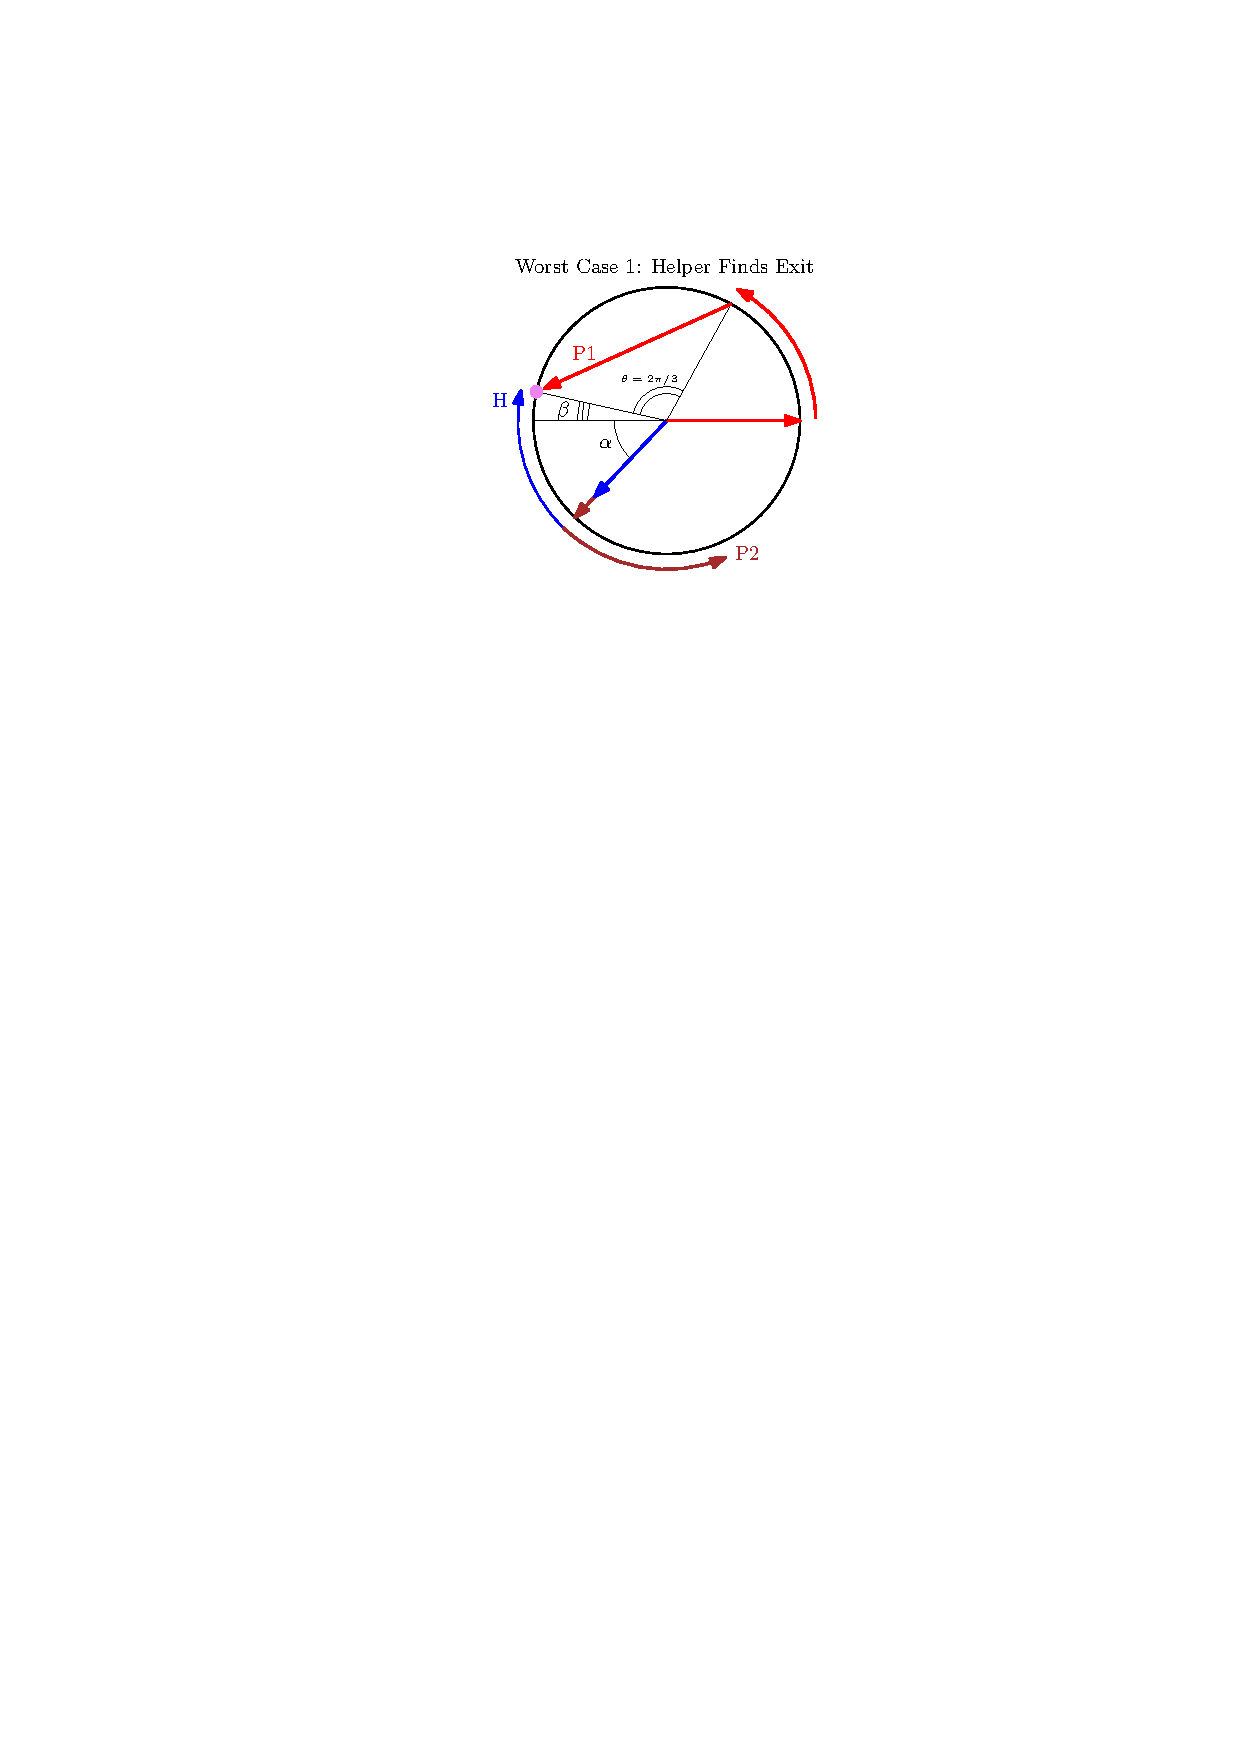
\includegraphics[width=\textwidth]{mypics/2Q1S_WorstCase_Servant.pdf}
                    %\caption{Figure 4}
                \end{subfigure}
                \begin{subfigure}{0.26\textwidth}
                    \centering
                    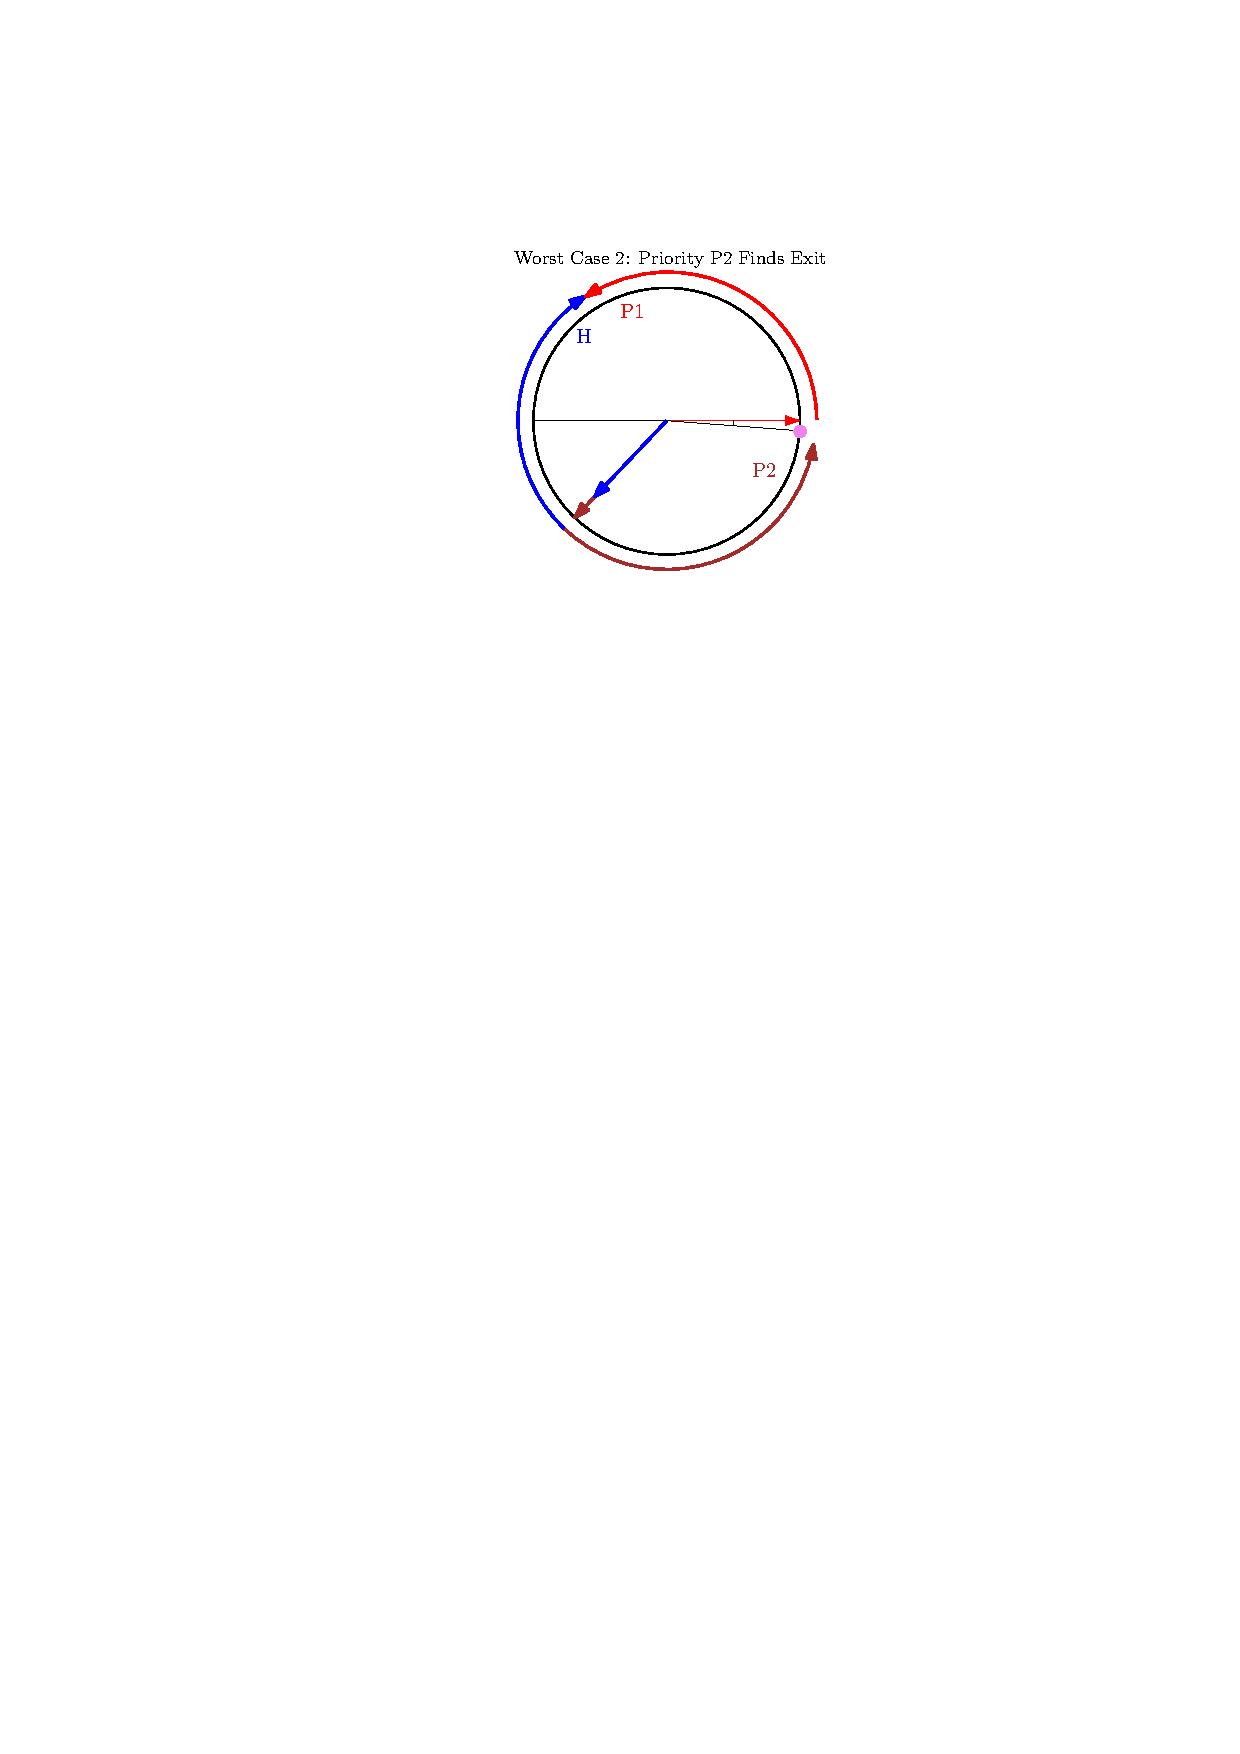
\includegraphics[width=\textwidth]{mypics/2Q1S_WorstCase_Priority.pdf}
                    %\caption{Figure 5}
                \end{subfigure}
                \hspace{0.1in}
                \begin{subfigure}{0.3\textwidth}
                    \centering
                    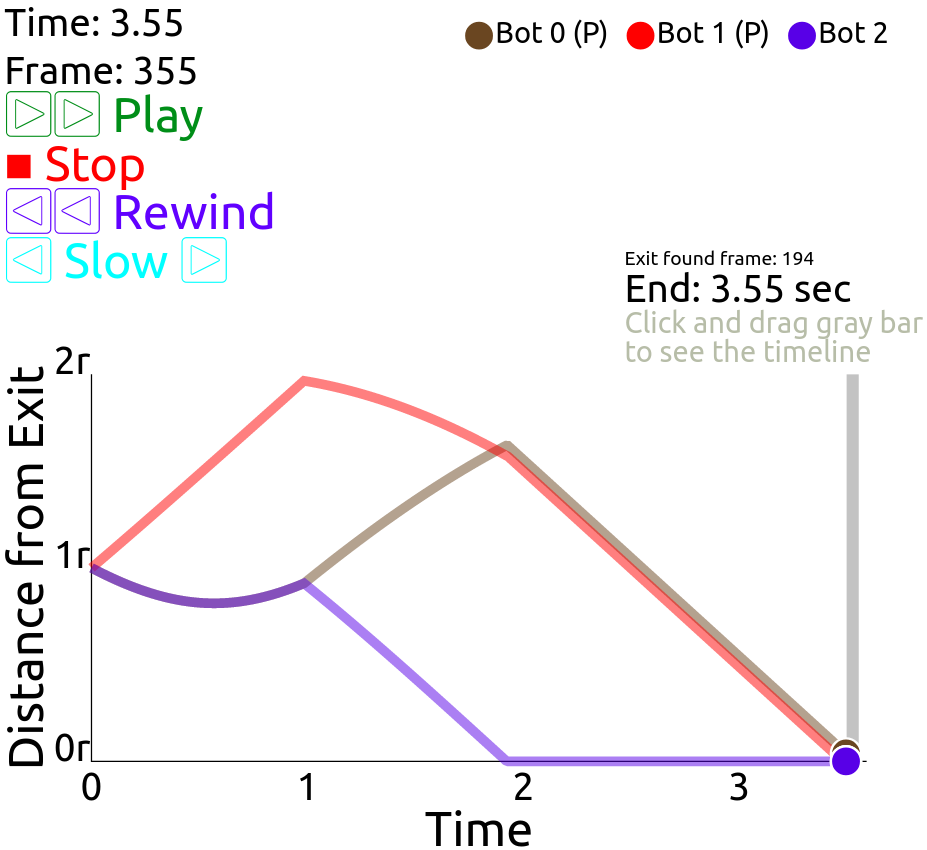
\includegraphics[width=\textwidth]{mypics/2Q1S_timeGraph.png}
                    %\caption{Figure 6}
                \end{subfigure}
            \end{figure}
            \vfill
            }


%%%%%%%%%%%%%%%%%%%%%%%%%%%%%%%%%%%%%%%%%%%%%%%%%%%%%%%%%%%%%%%%%%%%%%%%%%%%%%%%%%%%%%%%%%%%%%%%%%%%%%%%%%%%%%%%%%%%%%%%%%%%%%%%%%%%%%%%%%%
%%%%%%%%%%%%%%%%%%%%%%%%%%%%%%%%%%%         ALERT BLOCKS  FINISH                           %%%%%%%%%%%%%%%%%%%%%%%%%%%%%%%%%%%%%%%%%%%%%%%%
%%%%%%%%%%%%%%%%%%%%%%%%%%%%%%%%%%%%%%%%%%%%%%%%%%%%%%%%%%%%%%%%%%%%%%%%%%%%%%%%%%%%%%%%%%%%%%%%%%%%%%%%%%%%%%%%%%%%%%%%%%%%%%%%%%%%%%%%%%%









%%%%%%%%%%%%%%%%%%%%%%%%%%%%%%%%%%%%%%%%%%%%%%   TIPS  TO MAKE A NICE POSTER  %%%%%%%%%%%%%%%%%%%%%%%%%%%%%%%%%%%%%%%%%%%%%%%%%%%%%%%%%%%%%
% Common mistakes when compiling
% 1) There is an empty row in one of the blocks, remove it.
% 2) You forgot to close the brace } at the end of the block, close it.
% 3) The name of a block does not agree, for example you have \newSingle{Description}{\BlockDescription}
%                           and when you call it to form the main columns, you may have typed \SingleDescripption
%                           hence you should have typed  \SingleDescription, correct it.
% 4) It can not find a picture, perhaps you have it in the wrong folder.
% 5) Maybe it doesn't find mypostersettings.tex, it should be in the same folder as CoolPoster.tex
%
%
%%%%%  General Recomendations when typing your poster:
%%%%%  Your regular blocks MUST be short, two or three sentences each, see the examples above.
%%%%%  If your graph contains graphs, first genererate the pdf versions of each graph via LATEX,  then DVItoPS then PStoPDF
%%%%%                   as shown in the tex files contained in the folder mypics
%%%%%%%%%%%%%%%%%%%%%%%%%%%%%%%%%%%%%%%%%%%%%%%%%%%%%%%%   END OF TIPS  %%%%%%%%%%%%%%%%%%%%%%%%%%%%%%%%%%%%%%%%%%%%%%%%%%%%%%%%%%%%%%%%%%
